%	Name			:: 	sthlm Beamer Theme  HEAVILY based on the hsrmbeamer theme (Benjamin Weiss)
%	Author			:: 	Mark Hendry Olson (mark@hendryolson.com)
%	Created			::	2013-07-31
%	Updated	    	::	[[April]] 04, 2017 at 16:26:39
%	Version			:: 	2.0.2
%	Email			:: 	hendryolson@gmail.com
%	Website			:: 	http://markolson.se
%	Twitter			:: 	markolsonse
%	Instagram		:: 	markolsonse
%
%	License			:: 	This file may be distributed and/or modified under the
%					GNU Public License.
%
%	Description		::	This presentation is a demonstration of the sthlm beamer
%					theme, which is HEAVILY based on the HSRM beamer theme created by Benjamin Weiss
%					(benjamin.weiss@student.hs-rm.de), which can be found on GitHub
%					<https://github.com/hsrmbeamertheme/hsrmbeamertheme>.  It also borrows heavily
%					from the work of Matthias Vogelgesang, (https://bloerg.net) and his Metropolis Mtheme,
%					<https://github.com/matze/mtheme>.
%
%	Theme			::	newPxFont
%	Options			::	progressbar
%					::	sectionpages
%					::	numfooter
%					::	fullfooter
%					::	dovaligncolumns
%					::	protectframetitle
%					::	greybg
%					::	cblock
%					::	minimal


%-=-=-=-=-=-=-=-=-=-=-=-=-=-=-=-=-=-=-=-=-=-=-=-=
%
%        LOADING DOCUMENT
%
%-=-=-=-=-=-=-=-=-=-=-=-=-=-=-=-=-=-=-=-=-=-=-=-=

\documentclass[newPxFont,numfooter,sectionpages]{beamer}
\usepackage[utf8]{inputenc}
\usetheme{sthlm}
\usepackage{pgfplots}
\pgfplotsset{compat=1.14}
\usepackage{cancel}

%-=-=-=-=-=-=-=-=-=-=-=-=-=-=-=-=-=-=-=-=-=-=-=-=
%
%	PRESENTATION INFORMATION
%
%-=-=-=-=-=-=-=-=-=-=-=-=-=-=-=-=-=-=-=-=-=-=-=-=

\title{Stockholm Beamer Theme}
\subtitle{sthlm v2.0.2 is based on hsrm \& mTheme}
\date{\today}
\author{\texttt{MarkOlson.SE}}
\institute{Made in \textit{Sweden} \par \small{File: \jobname}}

\hypersetup{
pdfauthor = {Mark H. Olson: hendryolson@gmail.com},
pdfsubject = {Beamer},
pdfkeywords = {Beamer theme, sthlm},
pdfmoddate= {D:\pdfdate},
pdfcreator = {}
}

\begin{document}

%-=-=-=-=-=-=-=-=-=-=-=-=-=-=-=-=-=-=-=-=-=-=-=-=
%
%	TITLE PAGE
%
%-=-=-=-=-=-=-=-=-=-=-=-=-=-=-=-=-=-=-=-=-=-=-=-=

\maketitle

%-=-=-=-=-=-=-=-=-=-=-=-=-=-=-=-=-=-=-=-=-=-=-=-=
%	FRAME: Theme Package Requirements
%-=-=-=-=-=-=-=-=-=-=-=-=-=-=-=-=-=-=-=-=-=-=-=-=
\begingroup
\setbeamercolor{frametitle}{bg=\cnRed}
\setbeamercolor{normal text}{fg=\cnDarkGrey,bg=\cnLightRed}
\begin{frame}{Please use Metropolis Theme Instead}

Thank you for wanting to use sthlm.

\vspace{1em}

However, \textbf{you really should consider} using the Metropolis (mTheme) theme developed by Matthias Vogelgesang and the LaTeX community instead as it is very well maintained and documented.

\begin{center}
	\cBlue{\url{https://goo.gl/r683yn}}
\end{center}
\end{frame}
\endgroup


%-=-=-=-=-=-=-=-=-=-=-=-=-=-=-=-=-=-=-=-=-=-=-=-=
%
%	TABLE OF CONTENTS: OVERVIEW
%
%-=-=-=-=-=-=-=-=-=-=-=-=-=-=-=-=-=-=-=-=-=-=-=-=

\section*{Overview}
\begin{frame}{Overview}
% For longer presentations use hideallsubsections option
\tableofcontents[hideallsubsections]
\end{frame}

%-=-=-=-=-=-=-=-=-=-=-=-=-=-=-=-=-=-=-=-=-=-=-=-=
%
%	TABLE OF CONTENTS: OVERVIEW
%
%-=-=-=-=-=-=-=-=-=-=-=-=-=-=-=-=-=-=-=-=-=-=-=-=

\section{General Information}

%-=-=-=-=-=-=-=-=-=-=-=-=-=-=-=-=-=-=-=-=-=-=-=-=
%	FRAME:
%-=-=-=-=-=-=-=-=-=-=-=-=-=-=-=-=-=-=-=-=-=-=-=-=

\begin{frame}[c]{sthlm Theme Information}

\alert{sthlm} theme was originally designed to bring pdflatex support and color to the unique beamer \alert{hsrm} theme designed by Benjamin Weiss.  Thank You Ben!   

\begin{center}
\cBlue{\url{https://goo.gl/NRseuc}}
\end{center}

Since then, \alert{sthlm} has borrowed heavily from \alert{mTheme} developed by Matthias Vogelgesang.  

\end{frame}


%-=-=-=-=-=-=-=-=-=-=-=-=-=-=-=-=-=-=-=-=-=-=-=-=
%	FRAME:
%-=-=-=-=-=-=-=-=-=-=-=-=-=-=-=-=-=-=-=-=-=-=-=-=

\begin{frame}[c]{sthlm Theme Information}
	
\alert{sthlm} continues to be a theme that can easily be modified through the style files.  If you are looking for a packaged theme, then I highly recommend \alert{mTheme}.\\

\vspace{1em}

I use a custom version of \alert{sthlm} for daily decks and make a vanilla version of the theme available for others to use and modify. - Enjoy!

\end{frame}

%-=-=-=-=-=-=-=-=-=-=-=-=-=-=-=-=-=-=-=-=-=-=-=-=
%	FRAME:
%-=-=-=-=-=-=-=-=-=-=-=-=-=-=-=-=-=-=-=-=-=-=-=-=

\begin{frame}[c]{sthml Build Information}
\cRed{sthlm} theme has been designed and tested to work within the SageMathCloud (Linux) environment.\\

\vspace{1em}

\begin{alertblock}{Warning of Build Issues}
I cannot guarantee that the code used to create the sthlm theme is \emph{error free}, \emph{optimized}, \emph{well written} nor \emph{if it will work in your production environment}.
\end{alertblock}


\end{frame}

%-=-=-=-=-=-=-=-=-=-=-=-=-=-=-=-=-=-=-=-=-=-=-=-=
%	FRAME:
%-=-=-=-=-=-=-=-=-=-=-=-=-=-=-=-=-=-=-=-=-=-=-=-=

\begin{frame}[c]{Have Fun!}
If you have read this far, then you are probably interested in using / modifying this theme for your own project. \\
\vspace{1em}
Everything you need is in the

\begin{itemize}
	\item style files:
	\begin{itemize}
		\item \texttt{beamerthemesthlm.\cBlue{sty}},
		\item \texttt{beamerfontthemesthlm.\cBlue{sty}},
		\item \texttt{beamercolorthemesthlm.\cBlue{sty}}.
	\end{itemize}
\end{itemize}

\end{frame}

%-=-=-=-=-=-=-=-=-=-=-=-=-=-=-=-=-=-=-=-=-=-=-=-=
%	FRAME: WHERE TO GET
%-=-=-=-=-=-=-=-=-=-=-=-=-=-=-=-=-=-=-=-=-=-=-=-=

\begin{frame}[c]{Get it on GitHub}
This theme and all the documentation is hosted on GitHub \\
\vspace{1em}
\begin{center}
\large{Download, Fork, Contribute}

\cBlue{\url{https://goo.gl/0Wg6xt}}
\vspace{1em}

\begin{figure}
	\centerline{
\includegraphics[width=0.1\textwidth]{GitHub-Mark-120px-plus.png}}
\caption{Hosted on GitHub}
\end{figure}

\end{center}
\end{frame}

%-=-=-=-=-=-=-=-=-=-=-=-=-=-=-=-=-=-=-=-=-=-=-=-=
%	FRAME: Thank You Overleaf
%-=-=-=-=-=-=-=-=-=-=-=-=-=-=-=-=-=-=-=-=-=-=-=-=
\begingroup
\setbeamercolor{frametitle}{bg=\cnGreen}
\setbeamercolor{normal text}{fg=\cnDarkGrey,bg=\cnLightGreen}
\begin{frame}{Thank You Overleaf}

Special thank you to \cGreen{Overleaf} - especially \cGreen{Dr. Lian Tze Lim} for supporting those using the theme on Overleaf. Awesome work!

\vspace{1em}

You can view and download the theme from \cGreen{Overleaf}.

\begin{center}
	\cBlue{\url{https://goo.gl/Z5zrsF}}
\end{center}

\begin{figure}
	\centerline{
\includegraphics[width=0.7\textwidth]{overleaf.png}}
\caption{Thank You Overleaf}
\end{figure}


\end{frame}
\endgroup

%-=-=-=-=-=-=-=-=-=-=-=-=-=-=-=-=-=-=-=-=-=-=-=-=
%	FRAME:
%-=-=-=-=-=-=-=-=-=-=-=-=-=-=-=-=-=-=-=-=-=-=-=-=

\begin{frame}{Theme Package Requirements}

This theme requires that the following packages are installed:

\begin{columns}[t]
\begin{column}{0.5\textwidth}
\begin{itemize}
\item \emph{beamer}
\item \emph{backgrounds}
\item \emph{booktabs}
\item \emph{calc}
\end{itemize}
\end{column}

\begin{column}{0.5\textwidth}
\begin{itemize}
\item \emph{datetime}
\item \emph{ragged2e}
\item \emph{tikz}
\end{itemize}
\end{column}
\end{columns}
\vspace{1cm}
There is always the option of simplifying the theme to reduce the number of required packages. 

\end{frame}

%-=-=-=-=-=-=-=-=-=-=-=-=-=-=-=-=-=-=-=-=-=-=-=-=
%	FRAME:
%-=-=-=-=-=-=-=-=-=-=-=-=-=-=-=-=-=-=-=-=-=-=-=-=

\begin{frame}{Replace the Logo With Your Own}

The \cBlue{Sigtunaskolan Humanistiska Läroverket} logo, \texttt{logo.png}, should be replaced with your own.  I teach within the Mathematics Institution at SSHL.
\vspace{1cm}
\begin{figure}
	\centerline{
\includegraphics[width=0.3\textwidth]{logo.png}}
\caption{SSHL Logo}
\end{figure}

\end{frame}

%-=-=-=-=-=-=-=-=-=-=-=-=-=-=-=-=-=-=-=-=-=-=-=-=
%	FRAME: Theme Options
%-=-=-=-=-=-=-=-=-=-=-=-=-=-=-=-=-=-=-=-=-=-=-=-=

\begin{frame}{Theme Options}
\begin{table}[]
	\begin{tabularx}{\linewidth}{l>{\raggedright}X}
		\toprule
		\textbf{Option}			& \textbf{Description} \tabularnewline
		\midrule
		\texttt{\cBlue{newPxFont}} & newpxtext and newpxtext fonts will be used (pdfLaTeX) \tabularnewline
		\texttt{\cBlue{progressbar}} & Frame Title progress bar \tabularnewline
		\texttt{\cBlue{sectionpages}} & Section pages \tabularnewline
		\texttt{\cBlue{fullfooter}} & Footers with logo\tabularnewline
		\texttt{\cBlue{numfoooter}} & Footers with page number only \tabularnewline
		\texttt{\cBlue{greybg}} & Frame background default is set to grey \tabularnewline
		\texttt{\cBlue{cblock}} & Blocks with colored background \tabularnewline
		\texttt{\cBlue{protectFrameTitle}} & Protect the frame title (if needed) \tabularnewline
		\texttt{\cBlue{valigncolumns}} & Vertically align columns\tabularnewline
		\bottomrule
	\end{tabularx}
	\label{tab:options}
\end{table}
\end{frame}

%-=-=-=-=-=-=-=-=-=-=-=-=-=-=-=-=-=-=-=-=-=-=-=-=
%
%	SECTION: COLORS
%
%-=-=-=-=-=-=-=-=-=-=-=-=-=-=-=-=-=-=-=-=-=-=-=-=
\section{Colors}

%-=-=-=-=-=-=-=-=-=-=-=-=-=-=-=-=-=-=-=-=-=-=-=-=
%	FRAME:
%-=-=-=-=-=-=-=-=-=-=-=-=-=-=-=-=-=-=-=-=-=-=-=-=

\begin{frame}[c]{Color Style File}
	
The sthlm theme style file \texttt{beamerthemesthlm.sty} references the \texttt{beamercolorthemesthlm.sty} file for the theme colors automatically. \\
\vspace{1em}
If you wish to bring your own color theme, then you will have to either change the reference in the \texttt{beamerthemesthlm.sty} file or rename your style file to \texttt{beamercolorthemesthlm.sty}.

\end{frame}

%-=-=-=-=-=-=-=-=-=-=-=-=-=-=-=-=-=-=-=-=-=-=-=-=
%	FRAME:
%-=-=-=-=-=-=-=-=-=-=-=-=-=-=-=-=-=-=-=-=-=-=-=-=

\begin{frame}[c]{Primary Presentation Colors}

\begin{columns}[c]

%	Color Box: Dark Grey
\begin{column}{0.12\textwidth}
\vspace{3em}
\setbeamercolor{boxsthlmDarkGrey}{bg=\cnDarkGrey,fg=white}
\begin{beamercolorbox}[wd=\linewidth,ht=5ex,dp=3ex]{boxsthlmDarkGrey}
\centering
	\texttt{Grey}
\end{beamercolorbox}

\vspace{3em}

%	Color Box: Grey
\setbeamercolor{boxsthlmGrey}{bg=\cnGrey,fg=\cnDarkGrey}
\begin{beamercolorbox}[wd=\linewidth,ht=5ex,dp=3ex]{boxsthlmGrey}
\centering
	\texttt{Grey}
\end{beamercolorbox}

\end{column}

\begin{column}{0.12\textwidth}

\vspace{3em}
	
%	Color Box: Blue
\setbeamercolor{boxsthlmBlue}{bg=\cnBlue,fg=white}
\begin{beamercolorbox}[wd=\linewidth,ht=5ex,dp=3ex]{boxsthlmBlue}
\centering
	\texttt{Blue}
\end{beamercolorbox}

\vspace{3em}

%	Color Box: Light Blue
\setbeamercolor{boxsthlmLightBlue}{bg=\cnLightBlue,fg=\cnDarkGrey}
\begin{beamercolorbox}[wd=\linewidth,ht=5ex,dp=3ex]{boxsthlmLightBlue}
\centering
	\texttt{Blue}
\end{beamercolorbox}
\end{column}

\begin{column}{0.12\textwidth}

%	Color Box: Red
\vspace{3em}
\setbeamercolor{boxsthlmRed}{bg=\cnRed,fg=white}
\begin{beamercolorbox}[wd=\linewidth,ht=5ex,dp=3ex]{boxsthlmRed}
\centering
	\texttt{Red}
\end{beamercolorbox}

\vspace{3em}

%	Color Box: Light Red
\setbeamercolor{boxsthlmLightRed}{bg=\cnLightRed,fg=\cnDarkGrey}
\begin{beamercolorbox}[wd=\linewidth,ht=5ex,dp=3ex]{boxsthlmLightRed}
\centering
	\texttt{Red}
\end{beamercolorbox}
\end{column}

\begin{column}{0.12\textwidth}

\vspace{3em}

%	Color Box: Green
\setbeamercolor{boxsthlmGreen}{bg=\cnGreen,fg=white}
\begin{beamercolorbox}[wd=\linewidth,ht=5ex,dp=3ex]{boxsthlmGreen}
\centering
	\texttt{Green}
\end{beamercolorbox}

\vspace{3em}

%	Color Box: Light Green
\setbeamercolor{boxsthlmLightGreen}{bg=\cnLightGreen,fg=\cnDarkGrey}
\begin{beamercolorbox}[wd=\linewidth,ht=5ex,dp=3ex]{boxsthlmLightGreen}
\centering
	\texttt{Green}
\end{beamercolorbox}
\end{column}

\begin{column}{0.12\textwidth}

\vspace{3em}

%	Color Box: Purple
\setbeamercolor{boxsthlmPurple}{bg=\cnPurple,fg=white}
\begin{beamercolorbox}[wd=\linewidth,ht=5ex,dp=3ex]{boxsthlmPurple}
\centering
	\texttt{Purple}
\end{beamercolorbox}

\vspace{3em}

%	Color Box: Light Purple
\setbeamercolor{boxsthlmLightPurple}{bg=\cnLightPurple,fg=\cnDarkGrey}
\begin{beamercolorbox}[wd=\linewidth,ht=5ex,dp=3ex]{boxsthlmLightPurple}
\centering
	\texttt{Purple}
\end{beamercolorbox}
\end{column}

\begin{column}{0.12\textwidth}

\vspace{3em}

%	Color Box: Orange
\setbeamercolor{boxsthlmOrange}{bg=\cnOrange,fg=white}
\begin{beamercolorbox}[wd=\linewidth,ht=5ex,dp=3ex]{boxsthlmOrange}
\centering
	\texttt{Orange}
\end{beamercolorbox}

\vspace{3em}

%	Color Box: Light Orange
\setbeamercolor{boxsthlmLightOrange}{bg=\cnLightOrange,fg=\cnDarkGrey}
\begin{beamercolorbox}[wd=\linewidth,ht=5ex,dp=3ex]{boxsthlmLightOrange}
\centering
	\texttt{Orange}
\end{beamercolorbox}
\end{column}
\end{columns}
\end{frame}

%-=-=-=-=-=-=-=-=-=-=-=-=-=-=-=-=-=-=-=-=-=-=-=-=
%	FRAME:
%-=-=-=-=-=-=-=-=-=-=-=-=-=-=-=-=-=-=-=-=-=-=-=-=

\begin{frame}{Colored Text}
\begin{table}[]
	\caption{Colored Text}
	\begin{tabular}[]{lcc}
		\toprule
		Red				& \cLightRed{LightRed}	& \cRed{Red} 	\\[0.25em]
		Blue			& \cLightBlue{LightBlue}	& \cBlue{Blue}	\\[0.25em]
		Green			& \cLightGreen{LightGreen}	& \cGreen{Green}	\\[0.25em]
		Purple			& \cLightPurple{LightPurple}	& \cPurple{Purple}	\\[0.25em]
		Orange			& \cLightOrange{LightOrange}	& \cOrange{Orange}	\\[0.25em]
		Grey			& \cGrey{Grey}					& \cDarkGrey{DarkGrey}	\\[0.25em]
		\bottomrule
	\end{tabular}
	\label{tab:Colored Text}
\end{table}
\end{frame}

%-=-=-=-=-=-=-=-=-=-=-=-=-=-=-=-=-=-=-=-=-=-=-=-=
%	FRAME:
%-=-=-=-=-=-=-=-=-=-=-=-=-=-=-=-=-=-=-=-=-=-=-=-=
\begingroup
\setbeamercolor{background canvas}{bg=\cnGreen}
\begin{frame}{Frame Colored Backgrounds}

\centering{\cGrey{\Huge{Green Background}}}

\end{frame}
\endgroup

%-=-=-=-=-=-=-=-=-=-=-=-=-=-=-=-=-=-=-=-=-=-=-=-=
%	FRAME:
%-=-=-=-=-=-=-=-=-=-=-=-=-=-=-=-=-=-=-=-=-=-=-=-=
\begingroup
\setbeamercolor{background canvas}{bg=\cnLightGreen}
\begin{frame}{Frame Colored Backgrounds}


\centering{\Huge{Light Green Background}}


\end{frame}
\endgroup

%-=-=-=-=-=-=-=-=-=-=-=-=-=-=-=-=-=-=-=-=-=-=-=-=
%	FRAME: Theme Package Requirements
%-=-=-=-=-=-=-=-=-=-=-=-=-=-=-=-=-=-=-=-=-=-=-=-=
\begingroup
\setbeamercolor{frametitle}{bg=\cnGreen}
\begin{frame}[plain]{Colored Title Block}

\centering{\Huge{Great for examples}}


\end{frame}
\endgroup

%-=-=-=-=-=-=-=-=-=-=-=-=-=-=-=-=-=-=-=-=-=-=-=-=
%	FRAME:
%-=-=-=-=-=-=-=-=-=-=-=-=-=-=-=-=-=-=-=-=-=-=-=-=
\begingroup
\setbeamercolor{background canvas}{bg=\cnBlue}
\begin{frame}{Frame Colored Backgrounds}

\centering{\cGrey{\Huge{Blue Background}}}

\end{frame}
\endgroup

%-=-=-=-=-=-=-=-=-=-=-=-=-=-=-=-=-=-=-=-=-=-=-=-=
%	FRAME:
%-=-=-=-=-=-=-=-=-=-=-=-=-=-=-=-=-=-=-=-=-=-=-=-=
\begingroup
\setbeamercolor{background canvas}{bg=\cnLightBlue}
\begin{frame}{Frame Colored Backgrounds}

\centering{\Huge{Light Blue Background}}

\end{frame}
\endgroup

%-=-=-=-=-=-=-=-=-=-=-=-=-=-=-=-=-=-=-=-=-=-=-=-=
%	FRAME: Theme Package Requirements
%-=-=-=-=-=-=-=-=-=-=-=-=-=-=-=-=-=-=-=-=-=-=-=-=
\begingroup
\setbeamercolor{frametitle}{bg=\cnBlue}
\begin{frame}[plain]{Colored Title Block}

\centering{\Huge{Great for definitions}}


\end{frame}
\endgroup

%-=-=-=-=-=-=-=-=-=-=-=-=-=-=-=-=-=-=-=-=-=-=-=-=
%	FRAME:
%-=-=-=-=-=-=-=-=-=-=-=-=-=-=-=-=-=-=-=-=-=-=-=-=
\begingroup
\setbeamercolor{background canvas}{bg=\cnRed}
\begin{frame}{Frame Colored Backgrounds}

\centering{\cGrey{\Huge{Red Background}}}

\end{frame}
\endgroup

%-=-=-=-=-=-=-=-=-=-=-=-=-=-=-=-=-=-=-=-=-=-=-=-=
%	FRAME:
%-=-=-=-=-=-=-=-=-=-=-=-=-=-=-=-=-=-=-=-=-=-=-=-=
\begingroup
\setbeamercolor{background canvas}{bg=\cnLightRed}
\begin{frame}{Frame Colored Backgrounds}

\centering{\Huge{Light Red Background}}

\end{frame}
\endgroup

%-=-=-=-=-=-=-=-=-=-=-=-=-=-=-=-=-=-=-=-=-=-=-=-=
%	FRAME: Theme Package Requirements
%-=-=-=-=-=-=-=-=-=-=-=-=-=-=-=-=-=-=-=-=-=-=-=-=
\begingroup
\setbeamercolor{frametitle}{bg=\cnRed}
\begin{frame}[plain]{Colored Title Block}

\centering{\Huge{Great for alerts}}

\end{frame}
\endgroup

%-=-=-=-=-=-=-=-=-=-=-=-=-=-=-=-=-=-=-=-=-=-=-=-=
%	FRAME:
%-=-=-=-=-=-=-=-=-=-=-=-=-=-=-=-=-=-=-=-=-=-=-=-=
\begingroup
\setbeamercolor{background canvas}{bg=\cnPurple}
\begin{frame}{Frame Colored Backgrounds}

\centering{\cGrey{\Huge{Purple Background}}}

\end{frame}
\endgroup

%-=-=-=-=-=-=-=-=-=-=-=-=-=-=-=-=-=-=-=-=-=-=-=-=
%	FRAME:
%-=-=-=-=-=-=-=-=-=-=-=-=-=-=-=-=-=-=-=-=-=-=-=-=
\begingroup
\setbeamercolor{background canvas}{bg=\cnLightPurple}
\begin{frame}{Frame Colored Backgrounds}

\centering{\Huge{Light Purple Background}}
\end{frame}
\endgroup

%-=-=-=-=-=-=-=-=-=-=-=-=-=-=-=-=-=-=-=-=-=-=-=-=
%	FRAME: Theme Package Requirements
%-=-=-=-=-=-=-=-=-=-=-=-=-=-=-=-=-=-=-=-=-=-=-=-=
\begingroup
\setbeamercolor{frametitle}{bg=\cnPurple}
\begin{frame}[plain]{Colored Title Block}

\centering{\Huge{Great for Proofs}}


\end{frame}
\endgroup

%-=-=-=-=-=-=-=-=-=-=-=-=-=-=-=-=-=-=-=-=-=-=-=-=
%	FRAME:
%-=-=-=-=-=-=-=-=-=-=-=-=-=-=-=-=-=-=-=-=-=-=-=-=
\begingroup
\setbeamercolor{frametitle}{bg=white, fg=\cnBlue}
\begin{frame}{Simple Frames}

\centering{\Huge{Keeping it Simple}}

\end{frame}
\endgroup

%-=-=-=-=-=-=-=-=-=-=-=-=-=-=-=-=-=-=-=-=-=-=-=-=
%	FRAME:
%-=-=-=-=-=-=-=-=-=-=-=-=-=-=-=-=-=-=-=-=-=-=-=-=
\begingroup
\setbeamercolor{background canvas}{bg=\cnLightBlue}
\begin{frame}[plain]

\centering{\Huge{Plain Frame}}

\end{frame}
\endgroup

%-=-=-=-=-=-=-=-=-=-=-=-=-=-=-=-=-=-=-=-=-=-=-=-=
%	FRAME:
%-=-=-=-=-=-=-=-=-=-=-=-=-=-=-=-=-=-=-=-=-=-=-=-=
\begingroup
\setbeamercolor{background canvas}{bg=\cnDarkGrey}
\begin{frame}[plain]

\centering{\cGrey{\Huge{Plain Frame}}}

\end{frame}
\endgroup

%-=-=-=-=-=-=-=-=-=-=-=-=-=-=-=-=-=-=-=-=-=-=-=-=
%	SECTION: Blocks
%-=-=-=-=-=-=-=-=-=-=-=-=-=-=-=-=-=-=-=-=-=-=-=-=

\section{Blocks}\label{Blocks}


%-=-=-=-=-=-=-=-=-=-=-=-=-=-=-=-=-=-=-=-=-=-=-=-=
%	FRAME: Blocks
%-=-=-=-=-=-=-=-=-=-=-=-=-=-=-=-=-=-=-=-=-=-=-=-=

\begin{frame}{Blocks}

\begin{block}{Block Title Here}
		Great for definitions
\end{block}

\begin{alertblock}{Alert Title Here}
		Great for definitions
\end{alertblock}

\begin{exampleblock}{Example Title Here}
		Great for examples
\end{exampleblock}
\end{frame}

%-=-=-=-=-=-=-=-=-=-=-=-=-=-=-=-=-=-=-=-=-=-=-=-=
%	FRAME: Blocks
%-=-=-=-=-=-=-=-=-=-=-=-=-=-=-=-=-=-=-=-=-=-=-=-=

\begin{frame}{Blocks}

\begin{block}{Block Title Here}
	\begin{itemize}
		\item point 1
		\item point 2
	\end{itemize}
\end{block}

\begingroup
\setbeamercolor{block title}{fg=white, bg=\cnBlue}
\setbeamercolor{block body}{bg=\cnLightBlue}
\begin{block}{Blue Colored Blocks}
	Produced by using the \texttt{cblock} theme option
\end{block}
\endgroup
\end{frame}

%-=-=-=-=-=-=-=-=-=-=-=-=-=-=-=-=-=-=-=-=-=-=-=-=
%	FRAME: Additional Blocks
%-=-=-=-=-=-=-=-=-=-=-=-=-=-=-=-=-=-=-=-=-=-=-=-=

\begin{frame}{Additional Blocks}
\begin{alertblock}{Alert Block}
	Highlight important information.
\end{alertblock}

\begingroup
\setbeamercolor{block title}{fg=white, bg=\cnRed}
\setbeamercolor{block body}{bg=\cnLightRed}
\begin{block}{Red Colored Blocks}
	Produced by using the \texttt{cblock} theme option
\end{block}
\endgroup
\end{frame}

%-=-=-=-=-=-=-=-=-=-=-=-=-=-=-=-=-=-=-=-=-=-=-=-=
%	FRAME: Additional Blocks
%-=-=-=-=-=-=-=-=-=-=-=-=-=-=-=-=-=-=-=-=-=-=-=-=

\begin{frame}{Additional Blocks}

\begin{exampleblock}{Example Block}
	Examples can be good.
\end{exampleblock}

\begingroup
\setbeamercolor{block title}{fg=white, bg=\cnGreen}
\setbeamercolor{block body}{bg=\cnLightGreen}
\begin{block}{Green Colored Blocks}
	Produced by using the \texttt{cblock} theme option
\end{block}
\endgroup

\end{frame}

%-=-=-=-=-=-=-=-=-=-=-=-=-=-=-=-=-=-=-=-=-=-=-=-=
%	FRAME: Blocks
%-=-=-=-=-=-=-=-=-=-=-=-=-=-=-=-=-=-=-=-=-=-=-=-=

\begin{frame}{Custom Blocks}
\begingroup
\setbeamercolor{block title}{fg=white, bg=\cnPurple}
\setbeamercolor{block body}{bg=\cnLightPurple}
\begin{block}{Purple customization}
	Using the theme colors to generate colored blocks.
\end{block}
\endgroup

\end{frame}

%-=-=-=-=-=-=-=-=-=-=-=-=-=-=-=-=-=-=-=-=-=-=-=-=
%
%	SECTION: FONTS
%
%-=-=-=-=-=-=-=-=-=-=-=-=-=-=-=-=-=-=-=-=-=-=-=-=
\section{Fonts}

%-=-=-=-=-=-=-=-=-=-=-=-=-=-=-=-=-=-=-=-=-=-=-=-=
%	FRAME: 
%-=-=-=-=-=-=-=-=-=-=-=-=-=-=-=-=-=-=-=-=-=-=-=-=

\begin{frame}[c]{No Special Fonts Required}

This theme was originally made to work with \texttt{pdflatex} and the default latex fonts.\\
\vspace{1em}
\cRed{sthlm} does comes with a \texttt{pdflatex} font option, \cRed{newPxFont}, which loads the following fonts:

\begin{itemize}
	\item \emph{newpxtext} for text
	\item \emph{cantarell} for sans-serif
	\item \emph{inconsolata} for sans-serif monospaced
	\item \emph{newpxmath} for math
\end{itemize}

Please refer to the \texttt{beamerfontthememsthlm.sty} for the package requirements.

\end{frame}


%-=-=-=-=-=-=-=-=-=-=-=-=-=-=-=-=-=-=-=-=-=-=-=-=
%
%	SECTION: ADDITIONAL FEATURES
%
%-=-=-=-=-=-=-=-=-=-=-=-=-=-=-=-=-=-=-=-=-=-=-=-=
\section{Features}

%-=-=-=-=-=-=-=-=-=-=-=-=-=-=-=-=-=-=-=-=-=-=-=-=
%	FRAME: Tables
%-=-=-=-=-=-=-=-=-=-=-=-=-=-=-=-=-=-=-=-=-=-=-=-=

\begin{frame}{Tables}
\begin{table}[]
	\caption{Selection of window function and their properties}
	\begin{tabular}[]{lrrr}
		\toprule
		\textbf{Window}			& \multicolumn{1}{c}{\textbf{First side lobe}}
		                    & \multicolumn{1}{c}{\textbf{3\,dB bandwidth}}
		                    & \multicolumn{1}{c}{\textbf{Roll-off}} \\
		\midrule
		Rectangular				& 13.2\,dB	& 0.886\,Hz/bin	& 6\,dB/oct		\\[0.25em]
		Triangular				& 26.4\,dB	& 1.276\,Hz/bin	& 12\,dB/oct	\\[0.25em]
		Hann					& 31.0\,dB	& 1.442\,Hz/bin	& 18\,dB/oct	\\[0.25em]
		Hamming					& 41.0\,dB	& 1.300\,Hz/bin	& 6\,dB/oct		\\
		\bottomrule
	\end{tabular}
	\label{tab:WindowFunctions}
\end{table}
\end{frame}

%-=-=-=-=-=-=-=-=-=-=-=-=-=-=-=-=-=-=-=-=-=-=-=-=
%	FRAME:
%-=-=-=-=-=-=-=-=-=-=-=-=-=-=-=-=-=-=-=-=-=-=-=-=

\begin{frame}[c]{Mathematics Step by Step}
Show $[x^n]'=nx^{n-1}$ by using first principles.
\begin{align*}
\visible<+->{f'(x) & = \displaystyle \lim_{\Delta x \to 0} \frac{f(x+\Delta x)-f(x)}{\Delta x} \\}
\visible<+->{&= \displaystyle \lim_{\Delta x \to 0} \frac{(\cRed{x+\Delta x})^n - (\cRed{x})^n}{\Delta x}\\}
\visible<+->{&= \displaystyle \lim_{\Delta x \to 0} \frac{\binom{n}{0}x^n\Delta x^0 +\binom{n}{1}x^{n-1}\Delta x^1 + \cdots + \binom{n}{n}x^0\Delta x^n - \cRed{x^n} }{\Delta x}\\}
\visible<+->{&= \displaystyle \lim_{\Delta x \to 0} \frac{\cRed{1}x^n(\cRed{1}) +\cRed{n}x^{n-1}\Delta x^1 + \cdots + \cRed{1}(\cRed{1})\Delta x^n - \cRed{x^n} }{\Delta x}\\}
\visible<+->{&= \displaystyle \lim_{\Delta x \to 0} \frac{\cRed{x^n} +nx^{n-1}\Delta x + \cdots + \Delta x^n - \cRed{x^n} }{\Delta x}\\}
\visible<+->{&= \displaystyle \lim_{\Delta x \to 0} \frac{\cancel{\cRed{\Delta x}} (nx^{n-1} + \cdots + \Delta x^{n-1} ) }{\cancel{\Delta x}}\\}
\visible<+->{&=nx^{n-1}}
\end{align*}

\end{frame}

%-=-=-=-=-=-=-=-=-=-=-=-=-=-=-=-=-=-=-=-=-=-=-=-=
%	FRAME: Formulas
%-=-=-=-=-=-=-=-=-=-=-=-=-=-=-=-=-=-=-=-=-=-=-=-=

\begin{frame}{Functions}
\begin{block}{Gaussian Probability Density Function}
\[
f \left(x \mid \mu, \sigma^2 \right) = \dfrac{1}{\sqrt{2 \sigma^2 \pi}} e^{- \dfrac{(x-\mu)^2}{2\sigma^2}}
\]
\end{block}
\end{frame}

%-=-=-=-=-=-=-=-=-=-=-=-=-=-=-=-=-=-=-=-=-=-=-=-=
%	FRAME: 
%-=-=-=-=-=-=-=-=-=-=-=-=-=-=-=-=-=-=-=-=-=-=-=-=

\begin{frame}[c]{More Mathematics}

\begin{columns}[c]
\begin{column}{0.5\textwidth}
\begin{tikzpicture}[scale=0.7]
	\begin{axis}[
            domain=0:2, range=0:6,ymax=6,ymin=0,
            axis lines =left,
            every axis y label/.style={at=(current axis.above origin),anchor=south},
            every axis x label/.style={at=(current axis.right of origin),anchor=west},
            xtick={1,1.666}, ytick={1,3},
            xticklabels={$\cPurple{x}$,$\cPurple{x}+\cRed{\Delta x}$}, yticklabels={$f(\cPurple{x})$,$f(\cPurple{x}+\cRed{\Delta x})$},
            axis on top,
          ]
          \addplot [very thick,\cnRed, domain=(0:2)] {-1.994+2.994*x};S
	  	  \addplot [\cnDarkGrey,dashed] plot coordinates {(1,0) (1,1)};
          \addplot [\cnDarkGrey,dashed] plot coordinates {(0,1) (1,1)};
          \addplot [\cnDarkGrey,dashed] plot coordinates {(0,3) (1.666,3)};
          \addplot [\cnDarkGrey,dashed] plot coordinates {(1.666,0) (1.666,3)};
          \addplot [very thick,\cnBlue, smooth,domain=(0:1.833)] {-1/(x-2)};
          \addplot[color=\cnDarkGrey,fill=\cnDarkGrey,only marks,mark=*] coordinates{(1.666,3)};  %% closed hole
          \addplot[color=\cnDarkGrey,fill=\cnDarkGrey,only marks,mark=*] coordinates{(1,1)};  %% closed hole
        \end{axis}
\end{tikzpicture}
\end{column}

\begin{column}{0.5\textwidth}
\begin{align*}
m &= \frac{\Delta y}{\Delta x}	\\
\\
m & =  \frac{\visible<2->{f(\cPurple{x}+\cRed{\Delta x})}\visible<3->{-}\visible<4->{f(\cPurple{x})}}{\visible<5->{\cPurple{x}+\cRed{\Delta x}}\visible<6->{-}\visible<7->{\cPurple{x}}}\\
m  &=  \underbrace{\frac{\visible<8->{f(\cPurple{x}+\cRed{\Delta x})-f(\cPurple{x})}}{\visible<9->{\cRed{\Delta x}}}}_{\visible<10->{\text{\cRed{difference quotient}}}}
\end{align*}
\end{column}
\end{columns}

\visible<10->{The slope of the secant line }
\begin{itemize}
	\item<10-> can be found using the \cRed{difference quotient}
	\item<11-> represents a \cBlue{function}'s \cRed{average} slope on the interval $[\cPurple{x}, \cRed{x+\Delta x}]$
\end{itemize}

\end{frame}

%-=-=-=-=-=-=-=-=-=-=-=-=-=-=-=-=-=-=-=-=-=-=-=-=
%	FRAME:
%-=-=-=-=-=-=-=-=-=-=-=-=-=-=-=-=-=-=-=-=-=-=-=-=

\begin{frame}[c, fragile]{Fragile Frames Not a Problem}
\begin{tikzpicture}
	\begin{axis}[
            domain=0:6, range=0:7,
            ymin=-.2,ymax=7,
            width=\textwidth,
            height=7cm, %% Hard coded height! Moreover this effects the aspect ratio of the zoom--sort of BAD
            axis lines=none,
          ]
          \only<3->{\addplot [draw=none, fill=\cnDarkGrey!10!\cnGrey] plot coordinates {(.8,1.6) (2.834,5)} \closedcycle; %% zoom fill
          \addplot [draw=none, fill=\cnDarkGrey!10!\cnGrey] plot coordinates {(2.834,5) (4.166,5)} \closedcycle; %% zoom fill
          \addplot [draw=none, fill=white] plot coordinates {(1.2,1.6) (4.166,5)} \closedcycle; %% zoom fill
          \addplot [draw=none, fill=white] plot coordinates {(.8,1.6) (1.2,1.6)} \closedcycle; %% zoom fill
		  }
          \only<4->{\addplot [draw=none, fill=\cnDarkGrey!10!\cnGrey] plot coordinates {(3.3,3.6) (5.334,5)} \closedcycle; %% zoom fill
          \addplot [draw=none, fill=\cnDarkGrey!10!\cnGrey] plot coordinates {(5.334,5) (6.666,5)} \closedcycle; %% zoom fill
          \addplot [draw=none, fill=white] plot coordinates {(3.7,3.6) (6.666,5)} \closedcycle; %% zoom fill
          \addplot [draw=none, fill=white] plot coordinates {(3.3,3.6) (3.7,3.6)} \closedcycle; %% zoom fill
  }
          \only<4->{\addplot [draw=none, fill=\cnDarkGrey!10!\cnGrey] plot coordinates {(3.7,2.4) (6.666,1)} \closedcycle; %% zoom fill
          \addplot [draw=none, fill=\cnDarkGrey!10!\cnGrey] plot coordinates {(3.3,2.4) (3.7,2.4)} \closedcycle; %% zoom fill
          \addplot [draw=none, fill=white] plot coordinates {(3.3,2.4) (5.334,1)} \closedcycle; %% zoom fill
          \addplot [draw=none, fill=white] plot coordinates {(5.334,1) (6.666,1)} \closedcycle; %% zoom fill
 }

          \only<3->{\addplot [draw=none, fill=\cnDarkGrey!10!\cnGrey] plot coordinates {(.8,.4) (2.834,1)} \closedcycle; %% zoom fill
          \addplot [draw=none, fill=\cnDarkGrey!10!\cnGrey] plot coordinates {(2.834,1) (4.166,1)} \closedcycle; %% zoom fill
          \addplot [draw=none, fill=white] plot coordinates {(1.2,.4) (4.166,1)} \closedcycle; %% zoom fill
          \addplot [draw=none, fill=white] plot coordinates {(.8,.4) (1.2,.4)} \closedcycle; %% zoom fill
}
          \addplot[very thick,\cnRed, smooth,domain=(0:1.833)] {-1/(x-2)};
          \only<3->{\addplot[very thick,\cnRed, smooth,domain=(2.834:4.166)] {3.333/(2.050-.3*x)-0.333}; %% 2.5 to 4.333
          %\addplot[very thick,\cnRed, smooth,domain=(5.334:6.666)] {11.11/(1.540-.09*x)-8.109}; %% 5 to 6.833
          \only<4->\addplot[very thick,\cnRed, smooth,domain=(5.334:6.666)] {x-3}; %% 5 to 6.833
 }
         \only<2->{ \addplot[color=\cnRed,fill=\cnRed,only marks,mark=*] coordinates{(1,1)};}  %% point to be zoomed
          \only<3->{\addplot[color=\cnRed,fill=\cnRed,only marks,mark=*] coordinates{(3.5,3)}; } %% zoomed pt 1
          \only<4->{\addplot[color=\cnRed,fill=\cnRed,only marks,mark=*] coordinates{(6,3)}; } %% zoomed pt 2

          \addplot [->,\cnDarkGrey] plot coordinates {(0,0) (0,6)}; %% axis
          \addplot [->,\cnDarkGrey] plot coordinates {(0,0) (2,0)}; %% axis

          \only<2->{\addplot [\cnDarkGrey!50!\cnGrey] plot coordinates {(.8,.4) (.8,1.6)}; %% box around pt
          \addplot [\cnDarkGrey!50!\cnGrey] plot coordinates {(1.2,.4) (1.2,1.6)}; %% box around pt
          \addplot [\cnDarkGrey!50!\cnGrey] plot coordinates {(.8,1.6) (1.2,1.6)}; %% box around pt
          \addplot [\cnDarkGrey!50!\cnGrey] plot coordinates {(.8,.4) (1.2,.4)}; %% box around pt
 }
          \only<3->{\addplot [\cnDarkGrey!50!\cnGrey] plot coordinates {(2.834,1) (2.834,5)}; %% zoomed box 1
          \addplot [\cnDarkGrey!50!\cnGrey] plot coordinates {(4.166,1) (4.166,5)}; %% zoomed box 1
          \addplot [\cnDarkGrey!50!\cnGrey] plot coordinates {(2.834,1) (4.166,1)}; %% zoomed box 1
          \addplot [\cnDarkGrey!50!\cnGrey] plot coordinates {(2.834,5) (4.166,5)}; %% zoomed box 1
}
          \only<4->{\addplot [\cnDarkGrey] plot coordinates {(3.3,2.4) (3.3,3.6)}; %% box around zoomed pt
          \addplot [\cnDarkGrey] plot coordinates {(3.7,2.4) (3.7,3.6)}; %% box around zoomed pt
          \addplot [\cnDarkGrey] plot coordinates {(3.3,3.6) (3.7,3.6)}; %% box around zoomed pt
          \addplot [\cnDarkGrey] plot coordinates {(3.3,2.4) (3.7,2.4)}; %% box around zoomed pt
}
          \only<4->{\addplot [\cnDarkGrey] plot coordinates {(5.334,1) (5.334,5)}; %% zoomed box 2
          \addplot [\cnDarkGrey] plot coordinates {(6.666,1) (6.666,5)}; %% zoomed box 2
          \addplot [\cnDarkGrey] plot coordinates {(5.334,1) (6.666,1)}; %% zoomed box 2
          \addplot [\cnDarkGrey] plot coordinates {(5.334,5) (6.666,5)}; %% zoomed box 2
}
          \node at (axis cs:2.4,0) [anchor=east] {$x$};
          \node at (axis cs:0,6.9) [anchor=north] {$y$};
        \end{axis}
\end{tikzpicture}
\end{frame}

%-=-=-=-=-=-=-=-=-=-=-=-=-=-=-=-=-=-=-=-=-=-=-=-=
%	FRAME: PGFPlots
%-=-=-=-=-=-=-=-=-=-=-=-=-=-=-=-=-=-=-=-=-=-=-=-=

\begin{frame}{PGFPlots Example}
	\begin{figure}[h]
		\centering
		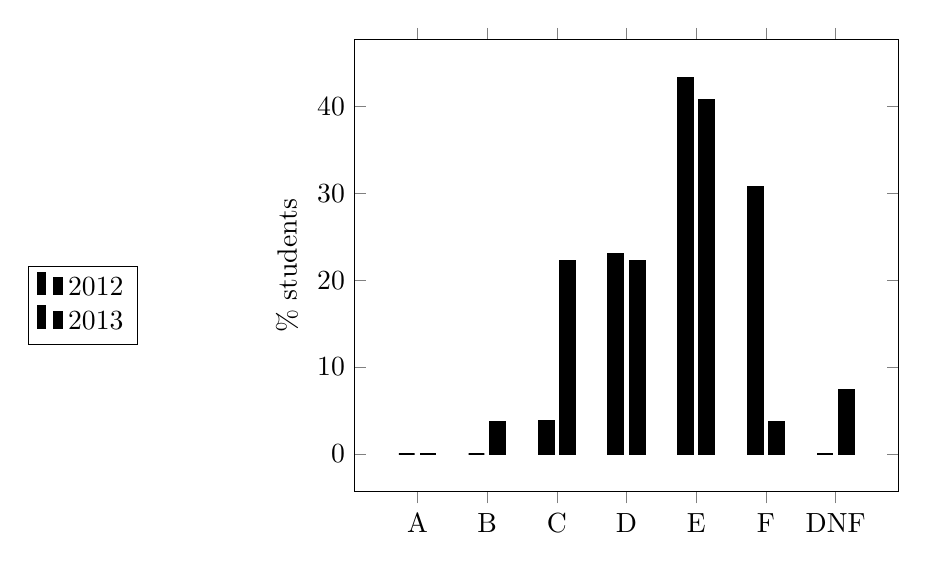
\begin{tikzpicture}
		\begin{axis}[
		    ybar,
		    enlarge x limits=0.15,
		    legend style={at={(-.5,0.5)},
		      anchor=north,legend columns=1},
		    ylabel={\% students},
		    symbolic x coords={A, B, C, D, E, F, DNF},
		    xtick=data,
		     bar width=2mm,
		     width=0.7\textwidth
		    ]
		    \legend{2012, 2013};
		    % Spring 2012 results
			\addplot[fill=\cnGrey]  coordinates {(A,0) (B,0) (C,3.85) (D,23.07) (E,43.31) (F,30.77) (DNF,0.00)};
			% Spring 2013 results
			\addplot[fill=\cnBlue]   coordinates {(A,0) (B,3.70) (C,22.22) (D,22.22) (E,40.74) (F,3.70) (DNF,7.41)};
		\end{axis}
		\end{tikzpicture}
		\caption{Consistent improvement over the last year}
		\end{figure}
\end{frame}

%-=-=-=-=-=-=-=-=-=-=-=-=-=-=-=-=-=-=-=-=-=-=-=-=
%	FRAME: Multiple Columns
%-=-=-=-=-=-=-=-=-=-=-=-=-=-=-=-=-=-=-=-=-=-=-=-=

\begin{frame}{Multiple Columns}
\begin{columns}
\begin{column}{.48\linewidth}
		Lorem ipsum dolor sit amet, consectetur adipisicing elit, sed do eiusmod
		tempor incididunt ut labore et dolore magna aliqua. Ut enim ad minim veniam.
\end{column}
\begin{column}{.48\linewidth}
		\begin{itemize}
        	\item Point 1
			\begin{itemize}
				\item Sub point a
				\item Sub point b
			\end{itemize}
        	\item Point 2
		\end{itemize}
	\end{column}
	\end{columns}
\end{frame}

\begin{frame}{References}
	\begin{thebibliography}{10}

	\beamertemplatebookbibitems
	\bibitem{Oppenheim2009}
	Alan V. Oppenheim
	\newblock Discrete - Time Signal Processing
	\newblock Prentice Hall Press, 2009

	\beamertemplatearticlebibitems
	\bibitem{EBU2011}
	European Broadcasting Union
	\newblock Specification of the Broadcast Wave Format (BWF)
	\newblock 2011

  \end{thebibliography}
\end{frame}

%-=-=-=-=-=-=-=-=-=-=-=-=-=-=-=-=-=-=-=-=-=-=-=-=
%
%	SECTION: Conclusion
%
%-=-=-=-=-=-=-=-=-=-=-=-=-=-=-=-=-=-=-=-=-=-=-=-=

\begin{frame}{About}

This sthlm beamer theme is free software: you can redistribute it and/or modify
it under the terms of the GNU General Public License as published by
the Free Software Foundation, either version 3 of the License, or
(at your option) any later version.\\
\vspace{1cm}
If you have any questions or comments
\begin{itemize}
	\item Website: \cBlue{markolson.se}
	\item Twitter: \cBlue{@markolsonse}
	\item Instagram: \cBlue{@markolson.se}
\end{itemize}
\end{frame}

%-=-=-=-=-=-=-=-=-=-=-=-=-=-=-=-=-=-=-=-=-=-=-=-=
%	FRAME:
%-=-=-=-=-=-=-=-=-=-=-=-=-=-=-=-=-=-=-=-=-=-=-=-=
\begingroup
\setbeamercolor{background canvas}{bg=\cnDarkGrey}
\begin{frame}[plain]

\centering{\cGrey{\Huge{THE \newline END}}}

\end{frame}
\endgroup

\end{document}